\section{Neurális hálók, kitekintés}

\subsubsection{Néhány kihívás és néhány megoldás mesterséges intelligencia segítségével}

\begin{itemize}
    \item nagy tömegű adat tárolása, visszakeresése
    \item beszéd előállítása
        \begin{itemize}
            \item Pocket - demo
        \end{itemize}
    \item természetes nyelv megértése
        \begin{itemize}
            \item Siri
            \item Google Asssistant
            \item Cortana
            \item Alexa
        \end{itemize}
    \item gépi fordítása
        \begin{itemize}
            \item Google Translate
        \end{itemize}
    \item alakfelismerés
        \begin{itemize}
            \item Face Unlock
        \end{itemize}
    \item robotvezérlés
        \begin{itemize}
            \item Boston Dynamics
        \end{itemize}
    \item zeneszerzés
    \item zenefelismerés
        \begin{itemize}
            \item Shazam
        \end{itemize}
\end{itemize}

\subsubsection{Példák gépi tanulásra}

\begin{itemize}
    \item spamszűrés
    \item karakterfelismerés
    \item fotók címkézése
    \item ajánló rendszerek
    \item szociális háló elemzése
    \item hírek csoportosítása témájuk alapján
\end{itemize}

\subsubsection{Alapfogalmak}

\begin{itemize}
    \item {\bf Tanuló adatbázis:} párok halmaza (pl. email-címke)
    \item {\bf Modell:} tudás ami alapján címkézhetünk
    \item {\bf Adatok:} e-mailek
    \item {\bf Információ az adatokról:} spam/nem spam címkékk
\end{itemize}

\begin{figure}[H]
    \centering
    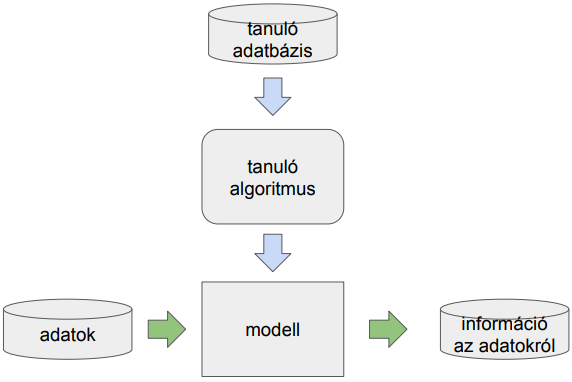
\includegraphics[width=0.8\textwidth]{gepi_tan_alapfogalmai}
    \caption{Gépi tanulás alapfogalmai}
    \label{fig:gepi_tan_alapfogalmai}
\end{figure}

{\bf Felügyelt} gépi tanulás esetén rendelkezésre állnak a közvetlen
információk. Pl.: spam/nem spam, karakterek, stb. (osztályozási feladatok).

{\bf Felügyelet nélküli} gépi tanulás esetén nincs közvetlen információ. Pl.:
csoportosítás/klaszterezés.

\begin{definicio}
    Regresszió.

    Az eredményváltozó hogyan függ a más (magyarázó) változók alakulásától.
    \begin{itemize}
        \item lineáris: $\hat{y} = a + bx$
            \begin{itemize}
                \item legkisebb négyzetek módszere
            \end{itemize}
        \item nem lineáris: $y = Ae^{Bx}$
        \item több osztályú problémák
    \end{itemize}
\end{definicio}

\begin{definicio}
    Osztályozás.

    Modell szeparáló egyenesek (hipersíkok).

    Módszerek:
    \begin{itemize}
        \item Bayes osztályozók
        \item Döntési fák
        \item Support Vector Machines
    \end{itemize}
\end{definicio}

\begin{definicio}
    Klaszterezés.

    \begin{itemize}
        \item Csoportok keresése - felügeylet nélküli tanulása
        \item Exkluzív (k-közép) vagy átfedő (fuzzy) módszer
        \item főkomponens analízás (PCA)
        \item hierarchikus
    \end{itemize}
\end{definicio}

\subsection{Neurális hálók és mélytanulás}

\subsubsection{Mesterséges neuronhálózat}

\begin{definicio}
    Neuron: számítási egység.
\end{definicio}

\begin{figure}[H]
    \centering
    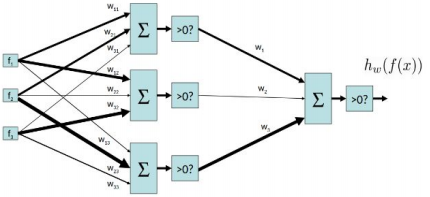
\includegraphics[width=0.8\textwidth]{neuronhalozat}
    \caption{Neuronhálózat}
    \label{fig:neuronhalozat}
\end{figure}

\begin{itemize}
    \item több $x_i$ bemenet (mindegyikhez $w_i$ súly rendelve)
    \item egy kimenet
        \begin{itemize}
            \item izgatottság: $\sum x_i w_i$
            \item ha az izgatottság túllép egy határszintet, akkor a neuron
                tüzel
        \end{itemize}
\end{itemize}

\begin{tetel}
    Egy kétszintű neuronhálózat elegendő számú neutronnal bármely folytonos
    függvényt képes megközelíteni tetszőleges pontossággal.
\end{tetel}

\begin{tetel}
    Mesterséges neuronhálózat szerkezete:

    \begin{itemize}
        \item teljesen kapcsolt réteg: \[
            H = XW + b
        \]
        \item  egyszerű konkurens réteg: \[
            H_t = XW_x + b_x + H_{t-1}W_h + b_h
        \]
        \item konvolúciós réteg: \[
            H = X * W + b
        .\]
        \item Aktivációs réteg: \[
            H = g(X)
        .\]
    \end{itemize}
\end{tetel}

Egy neuronhálózat tanítása számolásigényes feladat, a tanítás akár több hét is
lehet, az alkalmazás viszont gyors.

Tanítási módszerek:
\begin{itemize}
    \item hiba-visszaterjesztés
        \begin{itemize}
            \item az elvárt és kapott kimenet különbségénél megbecsüljük az egyes
                súlyok hozzájárulását a hibához
                \begin{itemize}
                    \item iránymenti deriváltak meghatározása, gradiens
                        irányban elmozdulás
                \end{itemize}
            \item az egyes súlyokat korrigáljuk ennek megfelelően (se túl kicsit, se túl sokat)
            \item zajos adatokkal nehezen boldogul
        \end{itemize}
    \item túltanulás elleni védekezés
        \begin{itemize}
            \item ritkítjuk a súlymátrixot (több $0$ érték)
            \item neuronok egy halmazát kirejti a hálózatból
        \end{itemize}
\end{itemize}

\subsubsection{Mélytanulás}

\begin{figure}[H]
    \centering
    \begin{tikzpicture}[scale=1,transform shape]
        \node[set,fill=blue!20,text width=5cm,label={[below=105pt of
            rea]mesterséges intelligencia}]
            (nat) at (0,-0.4)  (rea) {};
        \node[set,fill=red!20,text width=3cm,label={[below=60pt of int]gépi tanulás}]
            (int) at (0,-0.2)  {};
        \node[set,fill=olive!20,text width=1.5cm] (nat) at (0,0) {mélytanulás};
    \end{tikzpicture}
    \caption{A mélytanulás és a mesterséges intelligencia kapcsolata}
    \label{fig:hierarchia}
\end{figure}

A mélytanulást a következők teszik szükségessé:
\begin{itemize}
    \item Bonyolultabb feladatoknál a hagyományos módszerek rosszul
        teljesítenek (a jellemzők kinyerése nehéz munka).
    \item Amennyiben az input nagyobb méretű, a "keskeny" neuronhálózatok
        nem elegendőek
        \begin{itemize}
            \item a neuronok száma exponenciális növelendő
            \item a pontosság csapnivaló, a tanulás lassú
        \end{itemize}
\end{itemize}
